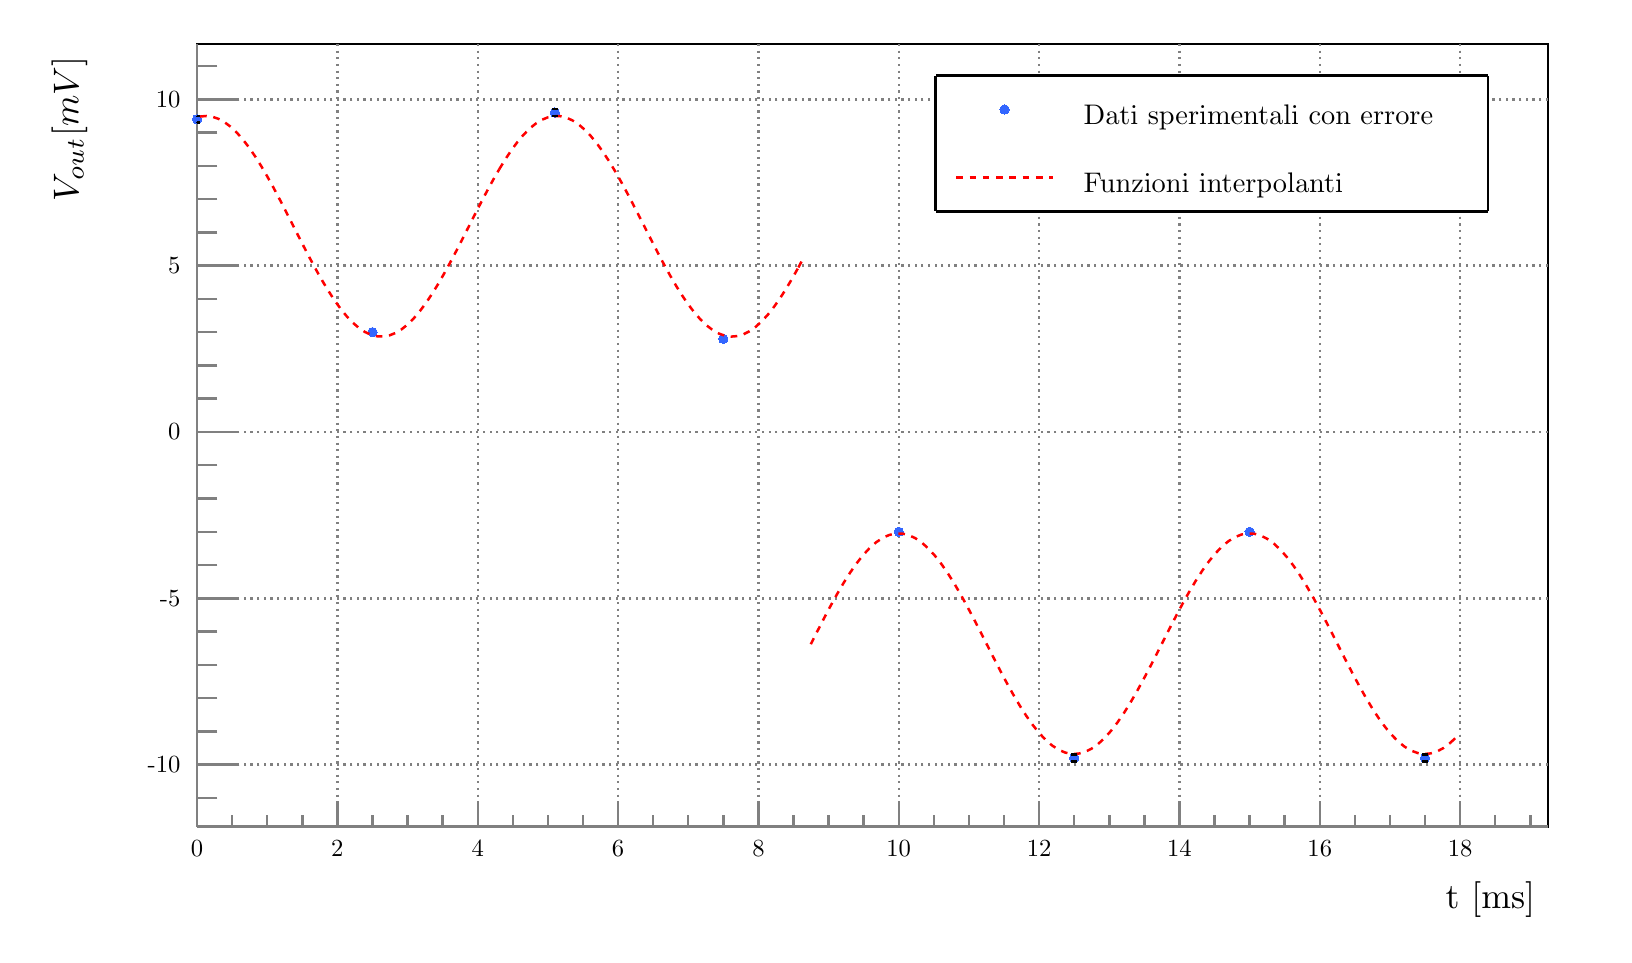
\begin{tikzpicture}
\pgfdeclareplotmark{cross} {
\pgfpathmoveto{\pgfpoint{-0.3\pgfplotmarksize}{\pgfplotmarksize}}
\pgfpathlineto{\pgfpoint{+0.3\pgfplotmarksize}{\pgfplotmarksize}}
\pgfpathlineto{\pgfpoint{+0.3\pgfplotmarksize}{0.3\pgfplotmarksize}}
\pgfpathlineto{\pgfpoint{+1\pgfplotmarksize}{0.3\pgfplotmarksize}}
\pgfpathlineto{\pgfpoint{+1\pgfplotmarksize}{-0.3\pgfplotmarksize}}
\pgfpathlineto{\pgfpoint{+0.3\pgfplotmarksize}{-0.3\pgfplotmarksize}}
\pgfpathlineto{\pgfpoint{+0.3\pgfplotmarksize}{-1.\pgfplotmarksize}}
\pgfpathlineto{\pgfpoint{-0.3\pgfplotmarksize}{-1.\pgfplotmarksize}}
\pgfpathlineto{\pgfpoint{-0.3\pgfplotmarksize}{-0.3\pgfplotmarksize}}
\pgfpathlineto{\pgfpoint{-1.\pgfplotmarksize}{-0.3\pgfplotmarksize}}
\pgfpathlineto{\pgfpoint{-1.\pgfplotmarksize}{0.3\pgfplotmarksize}}
\pgfpathlineto{\pgfpoint{-0.3\pgfplotmarksize}{0.3\pgfplotmarksize}}
\pgfpathclose
\pgfusepathqstroke
}
\pgfdeclareplotmark{cross*} {
\pgfpathmoveto{\pgfpoint{-0.3\pgfplotmarksize}{\pgfplotmarksize}}
\pgfpathlineto{\pgfpoint{+0.3\pgfplotmarksize}{\pgfplotmarksize}}
\pgfpathlineto{\pgfpoint{+0.3\pgfplotmarksize}{0.3\pgfplotmarksize}}
\pgfpathlineto{\pgfpoint{+1\pgfplotmarksize}{0.3\pgfplotmarksize}}
\pgfpathlineto{\pgfpoint{+1\pgfplotmarksize}{-0.3\pgfplotmarksize}}
\pgfpathlineto{\pgfpoint{+0.3\pgfplotmarksize}{-0.3\pgfplotmarksize}}
\pgfpathlineto{\pgfpoint{+0.3\pgfplotmarksize}{-1.\pgfplotmarksize}}
\pgfpathlineto{\pgfpoint{-0.3\pgfplotmarksize}{-1.\pgfplotmarksize}}
\pgfpathlineto{\pgfpoint{-0.3\pgfplotmarksize}{-0.3\pgfplotmarksize}}
\pgfpathlineto{\pgfpoint{-1.\pgfplotmarksize}{-0.3\pgfplotmarksize}}
\pgfpathlineto{\pgfpoint{-1.\pgfplotmarksize}{0.3\pgfplotmarksize}}
\pgfpathlineto{\pgfpoint{-0.3\pgfplotmarksize}{0.3\pgfplotmarksize}}
\pgfpathclose
\pgfusepathqfillstroke
}
\pgfdeclareplotmark{newstar} {
\pgfpathmoveto{\pgfqpoint{0pt}{\pgfplotmarksize}}
\pgfpathlineto{\pgfqpointpolar{44}{0.5\pgfplotmarksize}}
\pgfpathlineto{\pgfqpointpolar{18}{\pgfplotmarksize}}
\pgfpathlineto{\pgfqpointpolar{-20}{0.5\pgfplotmarksize}}
\pgfpathlineto{\pgfqpointpolar{-54}{\pgfplotmarksize}}
\pgfpathlineto{\pgfqpointpolar{-90}{0.5\pgfplotmarksize}}
\pgfpathlineto{\pgfqpointpolar{234}{\pgfplotmarksize}}
\pgfpathlineto{\pgfqpointpolar{198}{0.5\pgfplotmarksize}}
\pgfpathlineto{\pgfqpointpolar{162}{\pgfplotmarksize}}
\pgfpathlineto{\pgfqpointpolar{134}{0.5\pgfplotmarksize}}
\pgfpathclose
\pgfusepathqstroke
}
\pgfdeclareplotmark{newstar*} {
\pgfpathmoveto{\pgfqpoint{0pt}{\pgfplotmarksize}}
\pgfpathlineto{\pgfqpointpolar{44}{0.5\pgfplotmarksize}}
\pgfpathlineto{\pgfqpointpolar{18}{\pgfplotmarksize}}
\pgfpathlineto{\pgfqpointpolar{-20}{0.5\pgfplotmarksize}}
\pgfpathlineto{\pgfqpointpolar{-54}{\pgfplotmarksize}}
\pgfpathlineto{\pgfqpointpolar{-90}{0.5\pgfplotmarksize}}
\pgfpathlineto{\pgfqpointpolar{234}{\pgfplotmarksize}}
\pgfpathlineto{\pgfqpointpolar{198}{0.5\pgfplotmarksize}}
\pgfpathlineto{\pgfqpointpolar{162}{\pgfplotmarksize}}
\pgfpathlineto{\pgfqpointpolar{134}{0.5\pgfplotmarksize}}
\pgfpathclose
\pgfusepathqfillstroke
}
\definecolor{c}{rgb}{1,1,1};
\draw [color=c, fill=c] (0,0) rectangle (20,11.503);
\draw [color=c, fill=c] (2.14429,1.36273) rectangle (19.2986,11.3026);
\definecolor{c}{rgb}{0,0,0};
\draw [c,line width=0.9] (2.14429,1.36273) -- (2.14429,11.3026) -- (19.2986,11.3026) -- (19.2986,1.36273) -- (2.14429,1.36273);
\definecolor{c}{rgb}{1,1,1};
\draw [color=c, fill=c] (2.14429,1.36273) rectangle (19.2986,11.3026);
\definecolor{c}{rgb}{0,0,0};
\draw [c,line width=0.9] (2.14429,1.36273) -- (2.14429,11.3026) -- (19.2986,11.3026) -- (19.2986,1.36273) -- (2.14429,1.36273);
\definecolor{c}{rgb}{0.5,0.5,0.5};
\draw [c,line width=0.9] (2.14429,1.36273) -- (19.2986,1.36273);
\draw [c,dash pattern=on 0.80pt off 1.60pt ,line width=0.9] (2.14429,11.3026) -- (2.14429,1.36273);
\draw [c,dash pattern=on 0.80pt off 1.60pt ,line width=0.9] (3.92655,11.3026) -- (3.92655,1.36273);
\draw [c,dash pattern=on 0.80pt off 1.60pt ,line width=0.9] (5.70882,11.3026) -- (5.70882,1.36273);
\draw [c,dash pattern=on 0.80pt off 1.60pt ,line width=0.9] (7.49109,11.3026) -- (7.49109,1.36273);
\draw [c,dash pattern=on 0.80pt off 1.60pt ,line width=0.9] (9.27335,11.3026) -- (9.27335,1.36273);
\draw [c,dash pattern=on 0.80pt off 1.60pt ,line width=0.9] (11.0556,11.3026) -- (11.0556,1.36273);
\draw [c,dash pattern=on 0.80pt off 1.60pt ,line width=0.9] (12.8379,11.3026) -- (12.8379,1.36273);
\draw [c,dash pattern=on 0.80pt off 1.60pt ,line width=0.9] (14.6201,11.3026) -- (14.6201,1.36273);
\draw [c,dash pattern=on 0.80pt off 1.60pt ,line width=0.9] (16.4024,11.3026) -- (16.4024,1.36273);
\draw [c,dash pattern=on 0.80pt off 1.60pt ,line width=0.9] (18.1847,11.3026) -- (18.1847,1.36273);
\draw [c,dash pattern=on 0.80pt off 1.60pt ,line width=0.9] (18.1847,11.3026) -- (18.1847,1.36273);
\draw [c,line width=0.9] (2.14429,1.36273) -- (2.14429,11.3026);
\draw [c,dash pattern=on 0.80pt off 1.60pt ,line width=0.9] (19.2986,2.15046) -- (2.14429,2.15046);
\draw [c,dash pattern=on 0.80pt off 1.60pt ,line width=0.9] (19.2986,4.26284) -- (2.14429,4.26284);
\draw [c,dash pattern=on 0.80pt off 1.60pt ,line width=0.9] (19.2986,6.37521) -- (2.14429,6.37521);
\draw [c,dash pattern=on 0.80pt off 1.60pt ,line width=0.9] (19.2986,8.48758) -- (2.14429,8.48758);
\draw [c,dash pattern=on 0.80pt off 1.60pt ,line width=0.9] (19.2986,10.6) -- (2.14429,10.6);
\draw [c,dash pattern=on 0.80pt off 1.60pt ,line width=0.9] (19.2986,2.15046) -- (2.14429,2.15046);
\draw [c,dash pattern=on 0.80pt off 1.60pt ,line width=0.9] (19.2986,10.6) -- (2.14429,10.6);
\draw [c,line width=0.9] (2.14429,1.36273) -- (19.2986,1.36273);
\draw [c,line width=0.9] (2.14429,1.65871) -- (2.14429,1.36273);
\draw [c,line width=0.9] (2.58985,1.51072) -- (2.58985,1.36273);
\draw [c,line width=0.9] (3.03542,1.51072) -- (3.03542,1.36273);
\draw [c,line width=0.9] (3.48099,1.51072) -- (3.48099,1.36273);
\draw [c,line width=0.9] (3.92655,1.65871) -- (3.92655,1.36273);
\draw [c,line width=0.9] (4.37212,1.51072) -- (4.37212,1.36273);
\draw [c,line width=0.9] (4.81769,1.51072) -- (4.81769,1.36273);
\draw [c,line width=0.9] (5.26325,1.51072) -- (5.26325,1.36273);
\draw [c,line width=0.9] (5.70882,1.65871) -- (5.70882,1.36273);
\draw [c,line width=0.9] (6.15439,1.51072) -- (6.15439,1.36273);
\draw [c,line width=0.9] (6.59995,1.51072) -- (6.59995,1.36273);
\draw [c,line width=0.9] (7.04552,1.51072) -- (7.04552,1.36273);
\draw [c,line width=0.9] (7.49109,1.65871) -- (7.49109,1.36273);
\draw [c,line width=0.9] (7.93665,1.51072) -- (7.93665,1.36273);
\draw [c,line width=0.9] (8.38222,1.51072) -- (8.38222,1.36273);
\draw [c,line width=0.9] (8.82779,1.51072) -- (8.82779,1.36273);
\draw [c,line width=0.9] (9.27335,1.65871) -- (9.27335,1.36273);
\draw [c,line width=0.9] (9.71892,1.51072) -- (9.71892,1.36273);
\draw [c,line width=0.9] (10.1645,1.51072) -- (10.1645,1.36273);
\draw [c,line width=0.9] (10.6101,1.51072) -- (10.6101,1.36273);
\draw [c,line width=0.9] (11.0556,1.65871) -- (11.0556,1.36273);
\draw [c,line width=0.9] (11.5012,1.51072) -- (11.5012,1.36273);
\draw [c,line width=0.9] (11.9468,1.51072) -- (11.9468,1.36273);
\draw [c,line width=0.9] (12.3923,1.51072) -- (12.3923,1.36273);
\draw [c,line width=0.9] (12.8379,1.65871) -- (12.8379,1.36273);
\draw [c,line width=0.9] (13.2835,1.51072) -- (13.2835,1.36273);
\draw [c,line width=0.9] (13.729,1.51072) -- (13.729,1.36273);
\draw [c,line width=0.9] (14.1746,1.51072) -- (14.1746,1.36273);
\draw [c,line width=0.9] (14.6201,1.65871) -- (14.6201,1.36273);
\draw [c,line width=0.9] (15.0657,1.51072) -- (15.0657,1.36273);
\draw [c,line width=0.9] (15.5113,1.51072) -- (15.5113,1.36273);
\draw [c,line width=0.9] (15.9568,1.51072) -- (15.9568,1.36273);
\draw [c,line width=0.9] (16.4024,1.65871) -- (16.4024,1.36273);
\draw [c,line width=0.9] (16.848,1.51072) -- (16.848,1.36273);
\draw [c,line width=0.9] (17.2935,1.51072) -- (17.2935,1.36273);
\draw [c,line width=0.9] (17.7391,1.51072) -- (17.7391,1.36273);
\draw [c,line width=0.9] (18.1847,1.65871) -- (18.1847,1.36273);
\draw [c,line width=0.9] (18.1847,1.65871) -- (18.1847,1.36273);
\draw [c,line width=0.9] (18.6302,1.51072) -- (18.6302,1.36273);
\draw [c,line width=0.9] (19.0758,1.51072) -- (19.0758,1.36273);
\definecolor{c}{rgb}{0,0,0};
\draw [anchor=base] (2.14429,0.983126) node[scale=0.890168, color=c, rotate=0]{0};
\draw [anchor=base] (3.92655,0.983126) node[scale=0.890168, color=c, rotate=0]{2};
\draw [anchor=base] (5.70882,0.983126) node[scale=0.890168, color=c, rotate=0]{4};
\draw [anchor=base] (7.49109,0.983126) node[scale=0.890168, color=c, rotate=0]{6};
\draw [anchor=base] (9.27335,0.983126) node[scale=0.890168, color=c, rotate=0]{8};
\draw [anchor=base] (11.0556,0.983126) node[scale=0.890168, color=c, rotate=0]{10};
\draw [anchor=base] (12.8379,0.983126) node[scale=0.890168, color=c, rotate=0]{12};
\draw [anchor=base] (14.6201,0.983126) node[scale=0.890168, color=c, rotate=0]{14};
\draw [anchor=base] (16.4024,0.983126) node[scale=0.890168, color=c, rotate=0]{16};
\draw [anchor=base] (18.1847,0.983126) node[scale=0.890168, color=c, rotate=0]{18};
\draw [anchor= east] (19.2986,0.442485) node[scale=1.29074, color=c, rotate=0]{t [ms]};
\definecolor{c}{rgb}{0.5,0.5,0.5};
\draw [c,line width=0.9] (2.14429,1.36273) -- (2.14429,11.3026);
\draw [c,line width=0.9] (2.66276,2.15046) -- (2.14429,2.15046);
\draw [c,line width=0.9] (2.40352,2.57294) -- (2.14429,2.57294);
\draw [c,line width=0.9] (2.40352,2.99541) -- (2.14429,2.99541);
\draw [c,line width=0.9] (2.40352,3.41789) -- (2.14429,3.41789);
\draw [c,line width=0.9] (2.40352,3.84036) -- (2.14429,3.84036);
\draw [c,line width=0.9] (2.66276,4.26284) -- (2.14429,4.26284);
\draw [c,line width=0.9] (2.40352,4.68531) -- (2.14429,4.68531);
\draw [c,line width=0.9] (2.40352,5.10779) -- (2.14429,5.10779);
\draw [c,line width=0.9] (2.40352,5.53026) -- (2.14429,5.53026);
\draw [c,line width=0.9] (2.40352,5.95274) -- (2.14429,5.95274);
\draw [c,line width=0.9] (2.66276,6.37521) -- (2.14429,6.37521);
\draw [c,line width=0.9] (2.40352,6.79769) -- (2.14429,6.79769);
\draw [c,line width=0.9] (2.40352,7.22016) -- (2.14429,7.22016);
\draw [c,line width=0.9] (2.40352,7.64263) -- (2.14429,7.64263);
\draw [c,line width=0.9] (2.40352,8.06511) -- (2.14429,8.06511);
\draw [c,line width=0.9] (2.66276,8.48758) -- (2.14429,8.48758);
\draw [c,line width=0.9] (2.40352,8.91006) -- (2.14429,8.91006);
\draw [c,line width=0.9] (2.40352,9.33253) -- (2.14429,9.33253);
\draw [c,line width=0.9] (2.40352,9.75501) -- (2.14429,9.75501);
\draw [c,line width=0.9] (2.40352,10.1775) -- (2.14429,10.1775);
\draw [c,line width=0.9] (2.66276,10.6) -- (2.14429,10.6);
\draw [c,line width=0.9] (2.66276,2.15046) -- (2.14429,2.15046);
\draw [c,line width=0.9] (2.40352,1.72799) -- (2.14429,1.72799);
\draw [c,line width=0.9] (2.66276,10.6) -- (2.14429,10.6);
\draw [c,line width=0.9] (2.40352,11.0224) -- (2.14429,11.0224);
\definecolor{c}{rgb}{0,0,0};
\draw [anchor= east] (2.04429,2.15046) node[scale=0.890168, color=c, rotate=0]{-10};
\draw [anchor= east] (2.04429,4.26284) node[scale=0.890168, color=c, rotate=0]{-5};
\draw [anchor= east] (2.04429,6.37521) node[scale=0.890168, color=c, rotate=0]{0};
\draw [anchor= east] (2.04429,8.48758) node[scale=0.890168, color=c, rotate=0]{5};
\draw [anchor= east] (2.04429,10.6) node[scale=0.890168, color=c, rotate=0]{10};
\draw [anchor= east] (0.523046,11.3026) node[scale=1.29074, color=c, rotate=90]{$V_{out} [mV]$};
\definecolor{c}{rgb}{0.2,0.4,1};
\foreach \P in {(2.14429,10.3465), (4.37212,7.64263), (6.68907,10.431), (8.82779,7.55814), (11.0556,5.10779), (13.2835,2.23496), (15.5113,5.10779), (17.7391,2.23496)}{\draw[mark options={color=c,fill=c},mark size=1.681682pt, line width=0.000000pt,
 mark=*] plot coordinates {\P};}
\definecolor{c}{rgb}{1,0,0};
\draw [c,dash pattern=on 2.40pt off 2.40pt ,line width=0.9] (2.18305,10.3813) -- (2.26058,10.3884) -- (2.33811,10.3787) -- (2.41564,10.3524) -- (2.49317,10.3098) -- (2.5707,10.2515) -- (2.64822,10.178) -- (2.72575,10.0903) -- (2.80328,9.98948) --
 (2.88081,9.87667) -- (2.95834,9.75324) -- (3.03587,9.62067) -- (3.1134,9.48054) -- (3.19092,9.33452) -- (3.26845,9.18436) -- (3.34598,9.03185) -- (3.42351,8.87881) -- (3.50104,8.72706) -- (3.57857,8.57843) -- (3.6561,8.43468) -- (3.73362,8.29753) --
 (3.81115,8.16861) -- (3.88868,8.04948) -- (3.96621,7.94155) -- (4.04374,7.8461) -- (4.12127,7.76429) -- (4.1988,7.69708) -- (4.27632,7.64528) -- (4.35385,7.6095) -- (4.43138,7.59018) -- (4.50891,7.58755) -- (4.58644,7.60163) -- (4.66397,7.63226) --
 (4.7415,7.67907) -- (4.81902,7.7415) -- (4.89655,7.81881) -- (4.97408,7.91008) -- (5.05161,8.01421) -- (5.12914,8.12996) -- (5.20667,8.25596) -- (5.2842,8.39068) -- (5.36172,8.53254) -- (5.43925,8.67982) -- (5.51678,8.83078) -- (5.59431,8.98361) --
 (5.67184,9.13649) -- (5.74937,9.28759) -- (5.8269,9.4351) -- (5.90442,9.57727) -- (5.98195,9.7124);
\draw [c,dash pattern=on 2.40pt off 2.40pt ,line width=0.9] (5.98195,9.7124) -- (6.05948,9.83887) -- (6.13701,9.95517) -- (6.21454,10.0599) -- (6.29207,10.1519) -- (6.3696,10.2299) -- (6.44712,10.2931) -- (6.52465,10.3407) -- (6.60218,10.3722) --
 (6.67971,10.3871) -- (6.75724,10.3853) -- (6.83477,10.3668) -- (6.9123,10.3319) -- (6.98982,10.2809) -- (7.06735,10.2144) -- (7.14488,10.1333) -- (7.22241,10.0386) -- (7.29994,9.93124) -- (7.37747,9.81264) -- (7.455,9.68419) -- (7.53252,9.54742) --
 (7.61005,9.40396) -- (7.68758,9.25553) -- (7.76511,9.1039) -- (7.84264,8.95088) -- (7.92017,8.7983) -- (7.99769,8.64797) -- (8.07522,8.5017) -- (8.15275,8.36123) -- (8.23028,8.22824) -- (8.30781,8.10431) -- (8.38534,7.99093) -- (8.46287,7.88945) --
 (8.54039,7.80108) -- (8.61792,7.72688) -- (8.69545,7.66773) -- (8.77298,7.62434) -- (8.85051,7.59722) -- (8.92804,7.58671) -- (9.00557,7.59292) -- (9.08309,7.61578) -- (9.16062,7.65502) -- (9.23815,7.71018) -- (9.31568,7.78058) -- (9.39321,7.8654)
 -- (9.47074,7.96361) -- (9.54827,8.07405) -- (9.6258,8.1954) -- (9.70332,8.3262) -- (9.78085,8.4649);
\draw [c,dash pattern=on 2.40pt off 2.40pt ,line width=0.9] (9.78085,8.4649) -- (9.85838,8.60985);
\draw [c,dash pattern=on 2.40pt off 2.40pt ,line width=0.9] (9.93858,3.68057) -- (10.0215,3.84396) -- (10.1043,4.00521) -- (10.1872,4.16211) -- (10.2701,4.31252) -- (10.353,4.4544) -- (10.4358,4.58581) -- (10.5187,4.70495) -- (10.6016,4.81019) --
 (10.6845,4.90012) -- (10.7673,4.97349) -- (10.8502,5.0293) -- (10.9331,5.0668) -- (11.016,5.08547) -- (11.0988,5.08506) -- (11.1817,5.06557) -- (11.2646,5.02728) -- (11.3475,4.97069) -- (11.4303,4.89659) -- (11.5132,4.80598) -- (11.5961,4.7001) --
 (11.679,4.5804) -- (11.7618,4.44851) -- (11.8447,4.30622) -- (11.9276,4.15549) -- (12.0105,3.99836) -- (12.0933,3.83697) -- (12.1762,3.67354) -- (12.2591,3.51029) -- (12.342,3.34944) -- (12.4248,3.1932) -- (12.5077,3.04369) -- (12.5906,2.90295) --
 (12.6735,2.77291) -- (12.7563,2.65533) -- (12.8392,2.55182) -- (12.9221,2.4638) -- (13.005,2.39246) -- (13.0878,2.33878) -- (13.1707,2.30348) -- (13.2536,2.28706) -- (13.3365,2.28973) -- (13.4193,2.31146) -- (13.5022,2.35196) -- (13.5851,2.41066) --
 (13.668,2.48677) -- (13.7508,2.57925) -- (13.8337,2.68684) -- (13.9166,2.80807) -- (13.9995,2.94129);
\draw [c,dash pattern=on 2.40pt off 2.40pt ,line width=0.9] (13.9995,2.94129) -- (14.0824,3.08468) -- (14.1652,3.23628) -- (14.2481,3.39403) -- (14.331,3.55577) -- (14.4139,3.7193) -- (14.4967,3.88238) -- (14.5796,4.0428) -- (14.6625,4.19835) --
 (14.7454,4.34693) -- (14.8282,4.4865) -- (14.9111,4.61516) -- (14.994,4.73115) -- (15.0769,4.8329) -- (15.1597,4.91901) -- (15.2426,4.98831) -- (15.3255,5.03985) -- (15.4084,5.07293) -- (15.4912,5.0871) -- (15.5741,5.08217) -- (15.657,5.0582) --
 (15.7399,5.01552) -- (15.8227,4.95471) -- (15.9056,4.8766) -- (15.9885,4.78226) -- (16.0714,4.67298) -- (16.1542,4.55024) -- (16.2371,4.41572) -- (16.32,4.27125) -- (16.4029,4.11881) -- (16.4857,3.96048) -- (16.5686,3.79841) -- (16.6515,3.63482) --
 (16.7344,3.47194) -- (16.8172,3.31199) -- (16.9001,3.15715) -- (16.983,3.00953) -- (17.0659,2.87116) -- (17.1487,2.74391) -- (17.2316,2.62952) -- (17.3145,2.52955) -- (17.3974,2.44538) -- (17.4802,2.37813) -- (17.5631,2.32874) -- (17.646,2.29788) --
 (17.7289,2.28596) -- (17.8117,2.29316) -- (17.8946,2.31936) -- (17.9775,2.36422) -- (18.0604,2.42713);
\draw [c,dash pattern=on 2.40pt off 2.40pt ,line width=0.9] (18.0604,2.42713) -- (18.1432,2.50721);
\definecolor{c}{rgb}{0,0,0};
\draw [c,line width=0.9] (2.14429,10.3866) -- (2.14429,10.3892);
\draw [c,line width=0.9] (2.14429,10.3892) -- (2.18437,10.3892);
\draw [c,line width=0.9] (2.14429,10.3064) -- (2.14429,10.3037);
\draw [c,line width=0.9] (2.14429,10.3037) -- (2.18437,10.3037);
\draw [c,line width=0.9] (6.68907,10.471) -- (6.68907,10.4743);
\draw [c,line width=0.9] (6.64899,10.4743) -- (6.72915,10.4743);
\draw [c,line width=0.9] (6.68907,10.3909) -- (6.68907,10.3877);
\draw [c,line width=0.9] (6.64899,10.3877) -- (6.72915,10.3877);
\draw [c,line width=0.9] (13.2835,2.27504) -- (13.2835,2.27887);
\draw [c,line width=0.9] (13.2434,2.27887) -- (13.3235,2.27887);
\draw [c,line width=0.9] (13.2835,2.19488) -- (13.2835,2.19105);
\draw [c,line width=0.9] (13.2434,2.19105) -- (13.3235,2.19105);
\draw [c,line width=0.9] (17.7391,2.27504) -- (17.7391,2.27887);
\draw [c,line width=0.9] (17.699,2.27887) -- (17.7792,2.27887);
\draw [c,line width=0.9] (17.7391,2.19488) -- (17.7391,2.19105);
\draw [c,line width=0.9] (17.699,2.19105) -- (17.7792,2.19105);
\definecolor{c}{rgb}{1,1,1};
\draw [color=c, fill=c] (11.523,9.17836) rectangle (18.5371,10.9018);
\definecolor{c}{rgb}{0,0,0};
\draw [c,line width=0.9] (11.523,9.17836) -- (18.5371,9.17836);
\draw [c,line width=0.9] (18.5371,9.17836) -- (18.5371,10.9018);
\draw [c,line width=0.9] (18.5371,10.9018) -- (11.523,10.9018);
\draw [c,line width=0.9] (11.523,10.9018) -- (11.523,9.17836);
\draw [anchor=base west] (13.2766,10.2771) node[scale=1.02369, color=c, rotate=0]{Dati sperimentali con errore};
\definecolor{c}{rgb}{0.2,0.4,1};
\foreach \P in {(12.3998,10.4709)}{\draw[mark options={color=c,fill=c},mark size=1.681682pt, line width=0.000000pt, mark=*] plot coordinates {\P};}
\definecolor{c}{rgb}{0,0,0};
\draw [anchor=base west] (13.2766,9.41533) node[scale=1.02369, color=c, rotate=0]{Funzioni interpolanti};
\definecolor{c}{rgb}{1,0,0};
\draw [c,dash pattern=on 2.40pt off 2.40pt ,line width=0.9] (11.7861,9.60922) -- (13.0135,9.60922);
\end{tikzpicture}
